\chapter{Literature Review}
\label{ch:literaturereview}

This chapter reviews research and practice relevant to business continuity and the prioritization of critical-service recovery. Its concern is the path from an assessment of interruption impacts to recovery requirements, service priorities, and the dependencies that support delivery. The review therefore draws on business-continuity standards and government guidance, empirical and analytical work on business impact analysis (BIA), criticality and recovery planning, dependency models, decision-support systems (DSSs), and research methods for designing and evaluating information-system artifacts. The discussion distinguishes normative guidance, scholarly findings, and vendor descriptions because each supports a different kind of inference.

The chapter proceeds from the broader continuity-management context toward the particular analytical problem addressed by this project. Section~\ref{sec:lr_bcm} reviews business continuity management (BCM), relevant international standards, and Saudi national guidance. Section~\ref{sec:lr_bia} examines BIA, including impact categories, time-dependent assessment, recovery parameters, and analytical approaches. Section~\ref{sec:lr_prioritization} considers service criticality, recovery priorities, rule-based classifications, and the distinction between priority and executable recovery sequence. Section~\ref{sec:lr_dependencies} reviews service dependencies, interdependency models, and the assignment of criticality to supporting resources. Section~\ref{sec:lr_dss} discusses decision-support foundations, research prototypes, and documented continuity-management software. Section~\ref{sec:lr_methods} considers research and evaluation methods relevant to the proposed artifact. Section~\ref{sec:lr_gap} synthesizes the evidence and states the bounded research gap, and Section~\ref{sec:lr_summary} concludes the chapter.

The evidence base is purposive rather than exhaustive. It combines published research, public records for relevant standards, Saudi guidance supplied with the project, and public product documentation. The ISO discussion relies on public catalogue descriptions, not the full commercial standards; software comparisons rely on documentation rather than hands-on product tests; and individual case studies are interpreted within their stated settings. These boundaries are retained throughout the chapter so that documented features and reported results are not treated as broader validation than the available evidence permits.

\section{Business Continuity Management}
\label{sec:lr_bcm}

BCM addresses an organization's ability to continue prioritized activities and services when disruption affects people, facilities, technology, information, suppliers, or other operating conditions. It is not synonymous with information-technology disaster recovery. Disaster recovery typically concerns restoration of technology and data, whereas continuity management also considers the business activities and service outcomes that technology supports. Emergency response, crisis management, resilience, and risk management are related fields, but each emphasizes a different part of the organizational response. NIST's contingency-planning guidance makes this distinction operational by separating information-system contingency plans from business-continuity and continuity-of-operations plans, while explaining how business-process analysis informs system recovery priorities \cite{nist2010contingency}. In the Saudi National Framework, BCM is situated within a wider cycle of anticipation, assessment, prevention, continuity, preparedness, response, and recovery \cite{nrcnationalframework}.

The boundaries of the research field have not always been used consistently. Russo et al. observe variation in the ways business continuity and business continuity planning are defined across the literature they reviewed; their synthesis also demonstrates that BCM research draws on several neighboring disciplines and framework traditions \cite{russo2023maturity}. A reference-model study by Arias-Aranda et al. maps processes across continuity standards and guidance and verifies a proposed set of 22 BCMS processes with 39 German practitioners, including continuity managers and consultants \cite{bcms2026reference}. The panel recognized BIA and criticality analysis alongside incident handling, recovery, exercises, and resource management. The study offers evidence that these activities are recognizable components of a BCMS process model. It does not establish that the proposed model is exhaustive for every sector, since the verification was based on a predefined list and a geographically bounded practitioner panel \cite{bcms2026reference}.

For this thesis, BCM is treated as the organizational management activity through which continuity capability is established and maintained. A business continuity management system (BCMS) is the set of interrelated processes used to direct and control that activity. Resilience is the broader capacity to anticipate, absorb, adapt to, and recover from disruption; continuity contributes to that capacity but does not exhaust it. This distinction is important for the proposed system: a decision-support artifact that organizes BIA results and recovery priorities can support a BCMS, but its implementation alone does not establish organizational resilience, operational readiness, or conformity to a management-system standard.

\subsection{Standards and Frameworks}
\label{sec:lr_standards}

International standards and government guidance establish the place of BIA and recovery planning within BCM, but their scope and level of prescription differ. ISO 22301:2019 is a requirements standard for establishing, implementing, maintaining, and continually improving a BCMS. ISO 22313:2020 provides guidance on applying ISO 22301 across organizations and contexts, and ISO/TS 22317:2021 addresses the conduct of a documented BIA. The public catalogue description of ISO/TS 22317 states that the analysis should be adapted to organizational needs, objectives, resources, and constraints rather than following one mandatory method \cite{iso22301catalogue,iso22313catalogue,iso22317catalogue}. Since the full texts were not reviewed, no clause-level interpretation is made here.

NIST Special Publication 800-34 Rev. 1 is more operationally specific, although its scope is federal information-system contingency planning rather than comprehensive enterprise BCM. Its BIA process identifies business processes and their recovery criticality, identifies the information-system resources on which they rely, and sets recovery priorities for those resources \cite{nist2010contingency}. The guide distinguishes maximum tolerable downtime (MTD), the total outage a process can accept, from the recovery time objective (RTO), the target for restoring a supporting system resource. It explains that the RTO should normally be shorter than the MTD because post-restoration activities may consume additional time. The recovery point objective (RPO) concerns tolerable data loss and is not another duration to add to MTD \cite{nist2010contingency}. The guide's numerical scenarios and cost examples are illustrative, not prescribed thresholds.

The standards and NIST guide provide a conceptual and procedural foundation rather than one universal calculation. ISO describes the management-system and BIA scope; NIST provides process steps and definitions for system contingency planning. Neither public catalogue text nor the NIST guide supplies a generally applicable rule for converting an organization's time-indexed service impact ratings into one MTPD, an RTO, and a relative service priority. The Saudi materials are particularly relevant because they provide more concrete impact categories and recovery classifications while still leaving organizations discretion over important analytical choices.

\begin{table}[!t]
\centering
\caption{Standards and guidance documents compared by scope, treatment of business impact analysis, and nature of the requirements.}
\label{tab:lr_standards}
\footnotesize
\renewcommand{\arraystretch}{1.25}
\begin{tabularx}{\textwidth}{>{\raggedright\arraybackslash}p{2.6cm} >{\raggedright\arraybackslash}X >{\raggedright\arraybackslash}X >{\raggedright\arraybackslash}p{2.7cm}}
\toprule
\textbf{Document} & \textbf{Scope} & \textbf{Business impact analysis and recovery parameters} & \textbf{Nature of the text} \\
\midrule
ISO 22301:2019 \cite{iso22301catalogue} & Establishing and maintaining a business continuity management system suited to the organizational context. & Not stated in the published scope description. & Requirements standard. \\
ISO 22313:2020 \cite{iso22313catalogue} & Guidance on applying ISO 22301 to organizations of different types and contexts, so that delivery is sustained at a predefined acceptable capacity. & Not stated in the published scope description. & Guidance. \\
ISO/TS 22317:2021 \cite{iso22317catalogue} & Guidance on conducting a documented business impact analysis. & Adapts the analysis to organizational needs, objectives, resources, and constraints, and explicitly does not impose a single uniform process. & Technical specification (guidance). \\
NIST SP 800-34 Rev.~1 \cite{nist2010contingency} & Contingency planning for federal information systems; comprehensive business-process continuity is outside its scope. & Three analysis tasks (process criticality, resources, recovery priorities). Defines MTD, RTO, and RPO, and states that the RTO should normally be shorter than the MTD. Times and costs in the guide are illustrative. & Guidance with templates and examples. \\
\bottomrule
\end{tabularx}
\par\smallskip
\footnotesize Note: The entries for the ISO documents are based on their public catalogue descriptions.
\end{table}

Table~\ref{tab:lr_standards} summarizes the scope and level of prescription that can be supported by the reviewed public descriptions. It should not be read as a clause-by-clause comparison of complete standards. The distinction between a requirements standard, implementation guidance, and a technical specification matters: the presence of a topic in a catalogue scope does not establish the exact procedures an organization must use to calculate each recovery parameter.

\subsection{National Guidance in Saudi Arabia}
\label{sec:lr_saudi}

Two Saudi documents frame the applied setting of the project. The National Framework for Risk, Emergency and Business Continuity Management, issued by the General Secretariat of the National Risk Council, positions BCM within a broader national resilience framework. The supplied business-continuity chapter describes a staged planning process that includes policy, scope, governance, roles, and performance indicators, and treats BIA as a key input to continuity arrangements \cite{nrcnationalframework}. The Digital Government Authority (DGA) guideline addresses risk management and BCM for digital government. The English issue and the Arabic issue have different identifiers and issue metadata; the analysis below uses the reviewed English issue for the impact matrix and the Arabic BCM extract where relevant, treating these as related versions of the DGA guidance rather than independent studies \cite{dga2025bcm,dga2025guidelineen}.

The National Framework describes an organization-led BIA process. It moves from identifying services and products to examining enabling processes, impact criteria, consequences over time, resumption timeframes, priorities, resources, and dependencies. Suggested impact categories include financial, legal and regulatory, reputational, beneficiary, operational, health and safety, and contractual consequences. The organization selects a suitable assessment approach and may collect information through interviews, workshops, and questionnaires. Time points are selected in light of the entity's activities. The listed outputs include MTPD, RTO, minimum business continuity objective (MBCO), and, where data recovery is relevant, RPO. The document gives example recovery classes, but presents them as illustrative rather than compulsory values \cite{nrcnationalframework}. It also differentiates one-way and mutual dependencies and identifies upstream, internal, and downstream relationships, with dependency groupings that include physical, cyber or digital, geographic, and logical elements \cite{nrcnationalframework}.

The DGA guideline organizes management activities around a Plan--Do--Check--Act cycle and describes BIA as an assessment of operations, procedures, dependencies, and the consequences of disruption over time. An entity is expected to approve its impact matrix and record recovery requirements and enabling resources. The guidance notes that the assessment interval and starting point should reflect service sensitivity; a half-hour interval and a starting point measured in days are examples, not universal defaults. For digital platforms and applications, the guideline provides a five-level impact classification based on stakeholder, financial, legal and regulatory, and reputational factors. When factors indicate different levels, the highest level is selected, and the levels are associated with target recovery times of 4, 8, 12, 24, and 48 hours \cite{dga2025guidelineen}. These values clarify one government classification scheme; they should not be generalized to organizations outside its intended setting.

Together, the Saudi documents are explicit about the components of BIA and its expected outputs, and the DGA gives a documented rule for combining impact factors into a platform level. Both nevertheless leave organizations to approve their own criteria and time horizons. The DGA matrix assigns a level and target recovery time, but the reviewed passages do not specify how a series of ratings at successive time points should determine MTPD and RTO, how missing assessments should be handled, or how a dependency shared across services should inherit criticality. The National Framework requires dependencies to be mapped and considered but does not prescribe a single aggregation formula for the criticality of shared supporting resources \cite{nrcnationalframework,dga2025guidelineen}. These distinctions define the practical context for the BIA and prioritization literature reviewed next.

\section{Business Impact Analysis}
\label{sec:lr_bia}

BIA identifies the consequences of interruption for organizational activities and establishes the time-related requirements that inform continuity and recovery planning. It is the analytical stage most directly connected to the proposed TDRP methodology: TDRP takes service-level impact assessments as inputs and applies explicit rules to derive criticality, MTPD, RTO, and relative priorities. A BIA does not itself guarantee that an organization can achieve the recovery targets it records. Nor does it necessarily produce a sequence of restoration actions. Its outputs are assessments and requirements to be interpreted and used in subsequent planning.

\subsection{Assessment Units and Impact Categories}
\label{sec:lr_bia_process}

The unit of assessment varies across standards and applications. NIST SP 800-34 begins with business processes and examines the information-system resources that support them \cite{nist2010contingency}. The Saudi guidance addresses services, products, operations, platforms, and applications, while also relating them to enabling processes and resources \cite{nrcnationalframework,dga2025guidelineen}. Applied studies have used more specialized units. Horalek's metering case assessed groups of datasets and individual systems and assets in an automated meter-management environment; Budiyanto et al. examined the operation of a container terminal exposed to electricity disruption \cite{amm2023bia,container2021bia}. NIST IR 8286D likewise links essential products and processes to supporting assets and records impact values and their rationale in a BIA register \cite{quinn2025bia}. The selected unit affects the interpretation of every subsequent measure: a recovery target for a service, process, platform, and component does not describe the same decision.

Impact information is often elicited from people responsible for activities, supplemented where possible by operational or financial data. Horalek combined public technical materials with repeated guided interviews with dataset sponsors and owners, but the article does not report the respondent count or a measure of agreement among them \cite{amm2023bia}. Budiyanto et al. surveyed thirty commissioners, directors, and managers, reconciled reported impacts with management, and used a focus group to establish scales consistent with the terminal's objectives and risk preferences. The study also drew on operating records to compare productivity and throughput before and after an outage \cite{container2021bia}. These designs show that BIA can combine judgment and operational evidence; they also show that the quality of derived classifications depends on whose judgments are represented, how disagreements are resolved, and whether the adopted scale has observable anchors.

Impact categories are contextual rather than universal. The container-terminal study included loading and unloading productivity, economic loss, employee productivity, customer decline, reputation, and wasted energy. The metering study considered legal and contractual obligations, organizational operation, essential service provision, confidence and reputation, and financial loss, while separately classifying data in relation to confidentiality, integrity, and availability \cite{container2021bia,amm2023bia}. NIST IR 8286D presents mission, financial, and reputational impacts as examples that organizations should adapt, and distinguishes criticality associated with loss of availability from sensitivity associated with confidentiality or integrity \cite{quinn2025bia}. The shared implication is not that every organization should adopt identical categories, but that a usable method must make its categories, rating definitions, and aggregation rules explicit.

Case evidence also cautions against assuming that a defined scale automatically yields a reproducible classification. In the container-terminal paper, the reported classification for an eighteen-hour disruption is difficult to reconcile with the displayed thresholds for remaining throughput; an intermediate ratio appears to sit between the stated bands without an unambiguous mapping \cite{container2021bia}. Horalek's paper uses different numbers of grades in different presentations of its impact scale \cite{amm2023bia}. These observations concern the published cases, not BIA in general. They nonetheless illustrate a methodological requirement for rule-based DSSs: category boundaries, tie handling, missing values, and mappings from evidence to class should be documented and testable.

\subsection{Time-Dependent Impact Assessment}
\label{sec:lr_time_impact}

Time is central to BIA because the consequences of an interruption can accumulate or change as an outage persists. A time-indexed assessment records expected impact at selected durations rather than assigning one timeless rating to a service. The Saudi guidance explicitly allows assessment intervals to vary according to the sensitivity and operating context of the entity or service \cite{nrcnationalframework,dga2025guidelineen}. Research studies use several temporal representations, and these representations should not be conflated.

The metering case is among the more explicit examples of a time-indexed impact matrix. Horalek assesses availability impacts at seven durations, ranging from half an hour to more than a week, and applies the same criteria across the horizons. The resulting rows show how impact classifications change as the interruption lengthens. The paper interprets MTPD from the time band associated with high impact and identifies a separate period for medium impact \cite{amm2023bia}. The study reports different periods for individual systems, with values ranging from hours to more than a week. It also notes that the consequences of a given outage may depend on when it occurs relative to billing and reporting deadlines. Thus duration alone may not describe all temporal consequences \cite{amm2023bia}. At least one reported pair of high- and medium-impact periods is difficult to reconcile with the stated ordering of the thresholds, underlining the need for explicit validation of matrix outputs.

Other studies represent time differently. Budiyanto et al. examine an eighteen-hour electricity disruption and report that different impact dimensions follow different trajectories; reputational effects, for example, are discussed beyond the immediate interruption period \cite{container2021bia}. Von der Assen et al. represent persistent cyber-threat impact through loss per time frame and recovery level, while treating maximum tolerable disruption as an input to the calculation rather than deriving it from impact ratings \cite{vonderassen2024quanttm}. Sahebjamnia et al. model operational performance over discrete periods, using degraded operating levels and recovery trajectories in a joint continuity and recovery optimization model \cite{sahebjamnia2015integrated}. Aghabegloo et al. use an illustrative degradation-and-recovery profile as one part of an asset-criticality assessment \cite{assetcriticality2023}. In the latter optimization and criticality studies, time is a model variable, but the model is not the same as an organization eliciting service-impact thresholds at discrete horizons.

NIST criticality and risk guidance further emphasizes duration, operating condition, and mission effect. NIST IR 8179 asks analysts to consider how long an adverse condition persists before it becomes severe, while NIST IR 8286D recommends recording event timing and duration and accounting for partial loss of function \cite{nist2018criticality,quinn2025bia}. Commercial BIA documentation also describes impact ratings across configurable durations and rules for handling cases where no rating reaches the designated intolerable level; this is evidence about disclosed product behavior, not an independent evaluation of its effectiveness \cite{servicenow2025rto}.

Across these sources, time-indexed matrices and temporal loss trajectories are established analytical choices, but their outputs answer different questions. A trajectory of degraded service may support optimization; a loss curve can estimate financial exposure; a sequence of ordinal impact ratings can support an MTPD decision. Among the materials reviewed, relatively few specify how to select one threshold time from ratings observed only at discrete points, how to treat a missing time point, or how to respond when no observation reaches an unacceptable level. Where evidence falls between two assessed horizons, reporting an interval may be more defensible than implying a precise time not observed. Any rule that selects a point in that interval should be identified as a decision convention and evaluated accordingly.

\subsection{Recovery Parameters}
\label{sec:lr_parameters}

Several recovery terms describe distinct concepts. MTPD, also called MTD in some guidance, represents the period beyond which interruption consequences are unacceptable. RTO is a recovery target: the intended time to resume a service, process, or supporting system at a specified level. RPO is a data-loss tolerance, normally expressed as a point in time to which data must be restored. MBCO refers to a minimum level of service or activity to be maintained or resumed. An achieved recovery time is an observed result from an exercise or incident, not the same as a target. NIST, the National Framework, and DGA use different term sets and contexts, so terminology must be defined before values are compared \cite{nist2010contingency,nrcnationalframework,dga2025guidelineen}.

The relationship between tolerance and target varies in the reviewed approaches. The metering study constrains RTO by its assessed medium-impact period or MTPD and separately constrains RPO by the acceptable data-loss period; the tolerance limit is read from the time-indexed assessment, while the RTO remains a target chosen within that constraint \cite{amm2023bia}. The DGA guideline maps an impact tier to a target recovery time, whereas ServiceNow documentation describes a calculation using the smallest tolerated downtime across impact categories and a configured maximum for cases in which no category reaches the intolerable level \cite{dga2025guidelineen,servicenow2025rto}. These examples demonstrate that software and guidance can operationalize different rules; they do not establish one universally correct formula.

Sahebjamnia et al. take MTPD and a minimum operating objective from BIA as inputs to an optimization model and calculate operating and recovery trajectories under resource and budget constraints. This formulation illustrates that target requirements are not identical to the recovery plan that can be achieved when resources are limited \cite{sahebjamnia2015integrated}. Likewise, a plan's target is not proof of actual capability. The National Framework includes comparison of actual and target recovery times among indicative performance measures, while the case literature reviewed here offers limited evidence about whether proposed targets were achieved during real incidents \cite{nrcnationalframework,amm2023bia}. A sound information model should therefore preserve the distinction between assessed tolerance, planned target, minimum acceptable operation, data-loss tolerance, and observed result.

Terminology in analytical studies can depart from established usage. Sahebjamnia et al. use RPO in a sense related to operating level, while standards and most continuity guidance use RPO to describe tolerated data loss \cite{sahebjamnia2015integrated,nist2010contingency}. This thesis follows the latter usage and does not interpret an operational performance level as RPO.

Figure~\ref{fig:lr_temporal_parameters} presents a schematic example with invented values. Where ratings are collected only at discrete horizons, the exact time at which an impact crosses an unacceptable threshold is unknown; it falls between the last acceptable and first unacceptable observations. Horalek's use of a time band avoids false precision but leaves a decision about selecting a single MTPD value unresolved \cite{amm2023bia}. The figure makes this inference boundary explicit and motivates documenting how the proposed method handles it.

\begin{figure}[htbp]
\centering
\resizebox{0.95\textwidth}{!}{% Illustrative schematic only. Positions and ratings are not taken from any reviewed source.
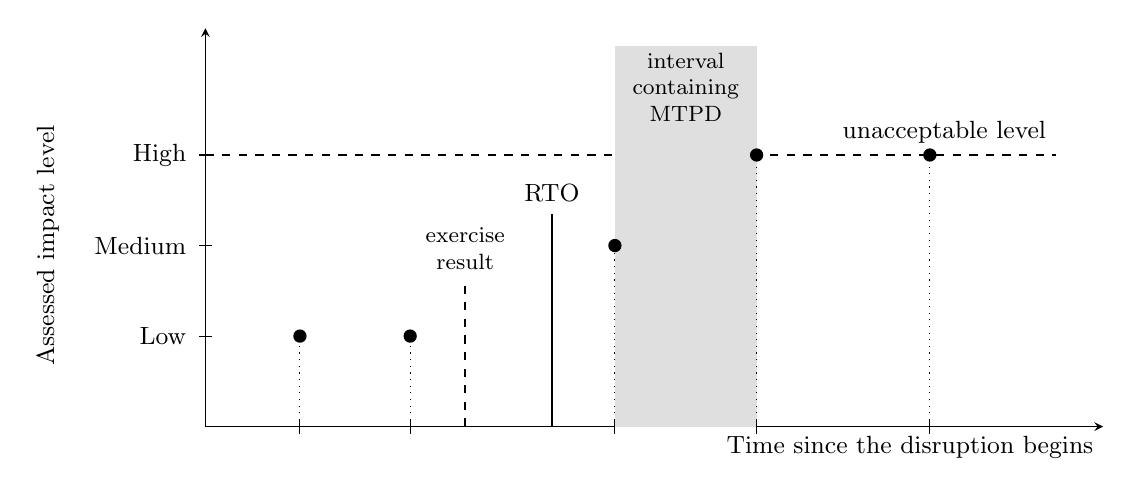
\begin{tikzpicture}[x=1cm,y=1.15cm,>=stealth,font=\small]
  % Axes
  \draw[->] (0,0) -- (11.4,0) node[below left] {Time since the disruption begins};
  \draw[->] (0,0) -- (0,4.4);
  \foreach \y/\l in {1/Low,2/Medium,3/High}{
    \draw (-0.08,\y) -- (0.08,\y);
    \node[left] at (-0.12,\y) {\l};
  }
  \node[rotate=90] at (-2.0,2) {Assessed impact level};
  % Unacceptable level
  \draw[dashed] (0,3) -- (10.8,3);
  \node[above left] at (10.8,3.02) {unacceptable level};
  % Interval that contains the MTPD
  \fill[gray!25] (5.2,0) rectangle (7.0,4.2);
  \node[align=center,font=\footnotesize] at (6.1,3.75) {interval\\containing\\MTPD};
  % Assessed points
  \foreach \x/\y in {1.2/1,2.6/1,5.2/2,7.0/3,9.2/3}{
    \fill (\x,\y) circle (2.4pt);
    \draw[dotted] (\x,0) -- (\x,\y);
    \draw (\x,-0.08) -- (\x,0.08);
  }
  % Recovery time objective and demonstrated recovery time
  \draw[thick] (4.4,0) -- (4.4,2.35);
  \node[above] at (4.4,2.38) {RTO};
  \draw[thick,dashed] (3.3,0) -- (3.3,1.6);
  \node[above,align=center,font=\footnotesize] at (3.3,1.63) {exercise\\result};
\end{tikzpicture}}
\caption{Schematic relation between assessed impact, the maximum tolerable period of disruption (MTPD), the recovery time objective (RTO), and the result of a recovery exercise. All positions and ratings are invented for illustration. When impact is assessed only at marked points, the shaded interval is the range in which the MTPD lies; selecting a single value within it requires an explicit rule.}
\label{fig:lr_temporal_parameters}
\end{figure}

\subsection{Analytical Approaches to BIA}
\label{sec:lr_bia_approaches}

The reviewed analytical approaches differ in their purpose and input requirements. Matrix-based approaches apply ordinal impact scales across activities or time horizons and may derive tolerability periods and recovery targets, as in Horalek's metering case \cite{amm2023bia}. Data-assisted approaches use operational records to calibrate or contextualize impact scales, as in the container-terminal study \cite{container2021bia}. Financial approaches estimate expected loss across threat and recovery scenarios, as in the QuantTM prototype; the maximum tolerable period remains an input in that model \cite{vonderassen2024quanttm}. Optimization approaches use tolerability limits and resource requirements to allocate operating levels and recovery effort over time \cite{sahebjamnia2015integrated}. Fuzzy multi-criteria and Bayesian approaches produce asset-criticality measures from expert weights and related indicators \cite{assetcriticality2023}. Process-mining approaches infer activity relationships from event logs and propagate scenario-dependent impacts through those relations \cite{raptaki2025propagation}. Table~\ref{tab:lr_bia_studies} compares representative studies by their objective, data, analytical technique, output, time treatment, and evaluation.

\begin{sidewaystable}[htbp]
\centering
\caption{Analytical studies on business impact analysis compared by objective, input data, technique, output, treatment of time, and evaluation.}
\label{tab:lr_bia_studies}
\footnotesize
\renewcommand{\arraystretch}{1.1}
\setlength{\tabcolsep}{4pt}
\begin{tabularx}{\linewidth}{>{\raggedright\arraybackslash}p{2.6cm} >{\raggedright\arraybackslash}X >{\raggedright\arraybackslash}X >{\raggedright\arraybackslash}X >{\raggedright\arraybackslash}X >{\raggedright\arraybackslash}X >{\raggedright\arraybackslash}X}
\toprule
\textbf{Study} & \textbf{Objective} & \textbf{Input data} & \textbf{Technique} & \textbf{Output} & \textbf{Treatment of time} & \textbf{Evaluation} \\
\midrule
Horalek (2023) \cite{amm2023bia} & Justify the protection of metering datasets and systems. & Technical material and repeated interviews with dataset owners; eleven system and asset entries. & Qualitative impact matrices by confidentiality, integrity, and availability class and business-impact criteria. & Impact ratings, MTPD, a medium-impact period, proposed RTO and RPO. & Availability rated at seven durations, from 30 minutes to more than a week. & One worked case; recovery outcomes not compared; respondents not reported. \\
Budiyanto et al. (2021) \cite{container2021bia} & Adapt BIA to electricity disruption at a container terminal. & Questionnaires with thirty managers, a focus group, and operating records before and after one disruption. & Management-approved five-level scales applied to remaining-capacity ratios. & Impact class in six categories; no MTPD or RTO. & One disruption of eighteen hours; reputation followed over later days. & One terminal; no independent comparison; one class mapping unclear. \\
Sahebjamnia et al. (2015) \cite{sahebjamnia2015integrated} & Integrate continuity and recovery planning under scarce resources. & MTPD and minimum objective from the BIA, AHP weights, resource needs, disruption likelihoods, budgets. & Multi-objective mixed-integer programming with an interactive epsilon-constraint method. & Operating-level trajectories, recovery times, resource allocations. & Discrete periods; non-decreasing recovery; minimum level after the tolerability deadline. & One manufacturer; hypothetical additional disruption. \\
Aghabegloo et al. (2023) \cite{assetcriticality2023} & Rank built physical assets by criticality with sustainability and resilience. & Expert judgements, site history, risk scenarios; product comparisons by four managers. & Fuzzy best--worst method, fuzzy TOPSIS, fuzzy DEMATEL, Bayesian network. & Asset criticality index and ranked contributors. & Recovery and restoration times as resilience factors; illustrative geometry. & One gas plant; face validity and sensitivity analysis; asset count reported inconsistently. \\
Von der Assen et al. (2024) \cite{vonderassen2024quanttm} & Express cyber-threat scenarios as expected financial loss. & Threat events, probabilities, durations, impact factors, recovery stages. & Probability-weighted loss over recovery stages in a browser prototype. & Expected loss per threat. & Recovery level per time frame; the maximum tolerable period is an input. & Preprint; one small firm; five-person focus group; no ground truth. \\
Raptaki et al. (2025) \cite{raptaki2025propagation} & Propagate cyber-incident impact across process activities. & Event log of one procurement process (553,763 events, 30 activities). & Process mining; weighted graph; iterative propagation; threshold of 0.5. & Scenario-dependent ranking of activities. & Relative scores; no tolerable period derived. & One company; five interviews; comparison with other propagation methods. \\
\bottomrule
\end{tabularx}
\end{sidewaystable}

These methods make different demands on the adopting organization. Sahebjamnia et al.'s optimization model requires importance weights, resource needs across operating levels, disruption likelihoods, and budgets; the case uses a defined product portfolio and disruption scenarios \cite{sahebjamnia2015integrated}. Aghabegloo et al.'s framework combines fuzzy weighting and ranking procedures with a Bayesian network built from expert judgment, and its structure depends on selected thresholds \cite{assetcriticality2023}. Raptaki et al. require process event logs; their case contains more than half a million events from one procurement process and uses a weighted graph to propagate impact among activities \cite{raptaki2025propagation}. By comparison, an ordinal matrix requires less quantitative infrastructure, but its reliability depends on clear scales and consistent elicitation.

The outputs are not interchangeable. A BIA matrix may yield a tolerability period or inform an RTO; a constrained optimization model may recommend operating trajectories and resource allocations; a criticality index yields a ranking; process mining yields relative, scenario-conditioned impact scores; and financial risk analysis yields expected-loss estimates. A ranking cannot substitute for an RTO, and neither automatically provides an executable restoration plan. Evaluation also varies: the studies include worked cases, hypothetical disruptions, sensitivity analyses, focus groups, and comparisons with other analytical techniques. They do not collectively demonstrate improved recovery performance in real incidents. Their evidence supports the feasibility and analytical plausibility of particular methods, while transferability and operational effectiveness remain open questions.

\section{Service Criticality and Recovery Prioritization}
\label{sec:lr_prioritization}

Criticality and recovery priority are related but distinct. Criticality characterizes the consequence or mission significance associated with losing a service, process, system, or asset. Recovery priority expresses the relative order or urgency assigned to restoration under stated criteria. An RTO is a time target, not a rank. A service can be highly critical but have a different recovery target from another service because its assessed impacts develop at a different rate. Conversely, two services can share a nominal target while competing for limited staff, facilities, or technology. The meaning of a priority therefore depends on the decision it is intended to support and the constraints it does not represent.

\subsection{Multi-Criteria and Criticality-Based Approaches}
\label{sec:lr_mcdm}

Multi-criteria decision-making approaches aggregate several dimensions into an index, class, or rank. Their attraction is that they can make trade-offs among mission, financial, safety, regulatory, service-user, and operational consequences visible. Their limitation is that rankings depend on the chosen attributes, scales, weights, and aggregation rule. When ratings are ordinal, arithmetic operations may imply distinctions that the scale does not justify; when weights are elicited from experts, they embody judgments that should be recorded and tested for sensitivity.

NIST IR 8179 presents a process model for criticality analysis that supports prioritizing systems and components in relation to mission and business functions. It emphasizes identifying important functions, the systems and components that enable them, and the consequences associated with degraded or unavailable capabilities; the resulting analysis informs risk and investment decisions \cite{nist2018criticality}. This form of criticality analysis is valuable as a structured trace from mission function to supporting technology. It is not itself a universal formula for time-dependent service MTPD or RTO. It also distinguishes ranking from the downstream decisions that allocate resources.

Aghabegloo et al. propose a quantitative framework for built physical-asset criticality that combines sustainability and resilience factors. Their case applies fuzzy best--worst weighting, fuzzy TOPSIS, fuzzy DEMATEL, and Bayesian-network analysis to expert judgments and asset information \cite{assetcriticality2023}. The work shows how a complex asset context can be represented through a multi-method criticality index, and it includes sensitivity analysis and face-validity discussion. Its unit of analysis is a built physical asset in a specific industrial setting, not a business service assessed across interruption time horizons. Its index therefore cannot be transferred directly to service recovery priority without defining a new mapping and testing its consequences.

The broader lesson is that a multi-criteria ranking should expose, rather than conceal, the criteria and weights on which it depends. It can help compare services when decision makers accept the measurement assumptions, but it does not automatically produce a recovery target, resolve a resource conflict, or describe dependencies among services. If the project uses a categorical or deterministic rule rather than weighted scoring, the same demand for transparency applies: users need to know which observations determined the classification and what happens at category boundaries.

\subsection{Rule-Based Prioritization}
\label{sec:lr_rules}

Rule-based methods express decision logic as explicit mappings from assessments to outputs. They can be easier to inspect and reproduce than complex models when the rules are small and deterministic, although their simplicity does not guarantee that the underlying thresholds are appropriate. Rule systems can also be configurable without making each organization's parameter values identical. The critical design questions include which inputs are mandatory, how different impact dimensions are combined, how discrete time bands map to tolerability and recovery targets, how conflicts are resolved, and how exceptions are surfaced to users.

The DGA impact matrix supplies a concrete example of categorical rule application: a platform is assigned to the highest indicated impact tier, which is associated with a stated recovery target \cite{dga2025guidelineen}. ServiceNow documentation describes a different configurable calculation in which category-specific impact downtimes are compared and a target is calculated from the minimum tolerated downtime, with a configured maximum used when no category reaches the intolerable level \cite{servicenow2025rto}. GlobalSuite documentation describes time-indexed service-impact tables and several ways to consolidate departmental BIA results, including average, weighted average, maximum, or minimum, as well as criteria for manual or automatic MTPD assignment \cite{globalsuite2025prebia}. GRASP documentation describes BIA assessments across configured time horizons and records recovery objectives, tolerability values, dependencies, and assessment rationale; the reviewed public material does not disclose a complete derivation algorithm for those parameters \cite{grasp2025bia}.

These examples establish that temporal assessments, tier mappings, consolidation rules, and configured thresholds are represented in existing guidance and software descriptions. They also demonstrate why comparison must examine the precise rule, not just the feature label. Choosing the highest impact tier, taking the minimum downtime, averaging departmental results, and allowing an analyst to set an RTO are materially different operations. Each entails a distinct interpretation of risk and may produce a different result from the same inputs. Vendor pages document claimed capabilities and disclosed procedures; they do not independently demonstrate the correctness or usability of those procedures.

For TDRP, a defensible rule set must state which impact assessments produce service criticality, which time point determines MTPD, how RTO is constrained in relation to the MTPD, what happens when the threshold is never reached, and how missing or contradictory values are treated. It should preserve the configuration that produced each output so that a practitioner can inspect the result and reproduce it. This is a design requirement for the proposed method, not a claim that prior research or products have never used configurable rules.

\subsection{Recovery Sequencing and Resource Constraints}
\label{sec:lr_sequencing}

A service priority is not equivalent to a feasible recovery sequence. Restoration may depend on shared infrastructure, technical prerequisites, staff availability, facilities, supplier actions, and minimum operating levels. A ranking says which services warrant greater urgency under the adopted criteria; it does not determine whether all high-priority services can be restored simultaneously or whether the systems supporting them can be recovered in the same order.

Sahebjamnia et al. integrate business continuity and disaster recovery planning through a multi-objective mixed-integer optimization model. It allocates scarce resources across operating levels and time periods while considering disruption scenarios, operational importance, recovery trajectories, and budgets \cite{sahebjamnia2015integrated}. This work makes explicit that recovery planning involves constrained allocation as well as relative importance. Its case study and hypothetical scenario demonstrate the model's operation but do not establish universal applicability across organizations or prove realized performance during incidents.

PRECESION addresses progressive recovery of interdependent services in enterprise data centers. El-Shekeil et al. model service dependencies and restoration capacity to determine staged recovery plans under constraints, contrasting a computed recovery plan with simply ranking services by individual importance \cite{elshekeil2017precesion}. The model is closer to technical restoration sequencing than a BIA decision-support dashboard. Its focus on interdependent data-center services and operational constraints is distinct from deriving service criticality from successive business-impact assessments.

The distinction shapes the scope of Masar. TDRP can provide prioritized services and related dependency information for human interpretation. Unless it represents operational constraints and computes a feasible schedule, its priority display should not be described as a restoration plan. Treating ranking and sequencing as separate outputs avoids implying that a nominal priority order can be executed without considering technical dependencies, resource limits, and incident-specific conditions.

\begin{sidewaystable}[htbp]
\centering
\caption{Representative approaches to criticality assessment, recovery planning, and impact propagation.}
\label{tab:lr_prioritization_methods}
\footnotesize
\renewcommand{\arraystretch}{1.15}
\setlength{\tabcolsep}{4pt}
\begin{tabularx}{\linewidth}{>{\raggedright\arraybackslash}p{2.8cm} >{\raggedright\arraybackslash}X >{\raggedright\arraybackslash}X >{\raggedright\arraybackslash}p{2.7cm} >{\raggedright\arraybackslash}X >{\raggedright\arraybackslash}X}
\toprule
\textbf{Approach} & \textbf{Unit and inputs} & \textbf{Decision logic} & \textbf{Output} & \textbf{Relation to time and dependencies} & \textbf{Evidence boundary} \\
\midrule
NIST criticality analysis \cite{nist2018criticality} & Mission and business functions, information systems, and supporting components. & Structured criticality analysis links system and component importance to the functions they enable. & Criticality information for risk and investment prioritization. & Links functions to supporting systems; considers duration and degraded operation, but does not prescribe service MTPD/RTO mapping. & Government process model; not an empirical validation of a universal recovery-priority formula. \\
Fuzzy asset criticality \cite{assetcriticality2023} & Built physical assets, expert assessments, site history, and resilience/sustainability factors. & Fuzzy best--worst weighting, TOPSIS, DEMATEL, and Bayesian network. & Asset criticality index and ranked contributors. & Recovery and restoration time enter as resilience factors; criterion relations are modeled, not service-to-resource inheritance. & One industrial case; authors report face validity and sensitivity analysis. \\
Integrated continuity and recovery optimization \cite{sahebjamnia2015integrated} & Products, operating levels, resource requirements, budgets, disruption likelihoods, and BIA tolerability inputs. & Multi-objective mixed-integer optimization with interactive solution exploration. & Operating trajectories, resource allocation, and recovery times. & Discrete-time recovery under resource constraints; consumes MTPD rather than deriving it from the time-indexed BIA. & One manufacturer case and an additional hypothetical disruption. \\
PRECESION recovery planning \cite{elshekeil2017precesion} & Interdependent enterprise data-center services and restoration constraints. & Progressive planning of service restoration under dependency and capacity constraints. & Staged recovery plan and service restoration order. & Explicitly models technical service dependencies; addresses sequence feasibility rather than service-level BIA derivation. & Model-based study in a data-center setting; not a general BCM maturity or BIA evaluation. \\
Process-mining propagation \cite{raptaki2025propagation} & Activities and event logs from one procurement process; incident scenarios. & Process mining constructs a weighted graph and propagates relative impact across activities. & Scenario-dependent relative impact scores and ranked activities. & Dependencies are inferred from event data; no MTPD or RTO is produced. & One company and process; reported results are not failure probabilities or universal dependency strengths. \\
Configured commercial rules \cite{servicenow2025rto,globalsuite2025prebia} & Service or category-level ratings across configured impact criteria and time horizons. & Product documentation describes minimum-downtime rules, maximum defaults, MTPD criteria, and alternative BIA consolidation options. & RTO and/or MTPD values and service classifications. & Time-indexed assessment is documented; dependency inheritance details vary and may not be disclosed. & Public vendor documentation only; no independent software test or comparative outcome study. \\
\bottomrule
\end{tabularx}
\end{sidewaystable}


Table~\ref{tab:lr_prioritization_methods} summarizes the differences among criticality analysis, multi-criteria ranking, optimization, and propagation approaches. Their distinct outputs make direct performance comparisons inappropriate without a common decision task and evaluation criteria.

\section{Dependency Modeling}
\label{sec:lr_dependencies}

Business services rely on networks of activities, people, facilities, applications, data, suppliers, and other resources. A service-first continuity analysis must therefore connect assessed services to the entities that enable them. A dependency map can explain why a service has particular recovery requirements, identify resources shared across services, and expose potential points of concentration. The map alone does not determine the criticality of a dependency or the order in which that dependency should be restored.

\subsection{Service Dependencies and Interdependencies}
\label{sec:lr_service_dependency}

Dependency models vary in direction, type, and scope. The National Framework distinguishes one-way and mutual relationships and describes upstream, internal, and downstream links. It also separates physical, cyber or digital, geographic, and logical dependencies \cite{nrcnationalframework}. The DGA guideline similarly calls for documenting dependencies among services, platforms, applications, people, systems, and facilities and identifies missing priority and dependency maps as continuity-planning weaknesses \cite{dga2025guidelineen}. These classifications are useful for BIA and recovery planning because the consequences of a service interruption may arise from both direct loss of the service and failure of a supporting element.

Rinaldi et al. provide a foundational conceptual account of interdependencies among critical infrastructures. They distinguish physical, cyber, geographic, and logical interdependencies and discuss how coupling, operating state, failure type, and infrastructure characteristics affect the propagation of disruption \cite{rinaldi2001interdependencies}. The framework is valuable for understanding that a dependency is not always a simple static edge: an effect may be direct or indirect, one-way or reciprocal, and conditioned by the state of the connected systems. Its focus is critical infrastructure at a system level, however, and its conceptual typology does not specify an organization-level formula for assigning a business service's criticality to each supporting asset.

NIST guidance also connects business functions with the systems and assets that enable them. NIST SP 800-34 asks analysts to identify system resources supporting business processes and set recovery priorities for those resources \cite{nist2010contingency}. NIST IR 8286D emphasizes retaining the rationale linking essential products and processes to assets and indicates that supporting assets derive priority from the functions they enable \cite{quinn2025bia}. This mission-to-asset traceability is relevant to service-first decision support, but the precise method for aggregating priority where one asset enables several functions still depends on the analysis and context.

Several analytical approaches infer dependencies from different evidence. Raptaki et al. use process-mining techniques to derive relationships among activities from an event log and propagate scenario-related impact through a weighted process graph \cite{raptaki2025propagation}. This can reveal relationships not recorded in static process descriptions, but the resulting scores are relative and scenario-dependent. The case covers one procurement process in one company, and its event-log relationships are not equivalent to system-failure probabilities, service MTPD, or universal dependency strengths \cite{raptaki2025propagation}. Aghabegloo et al.'s fuzzy DEMATEL and Bayesian components likewise model relations among criteria and asset factors; these criterion relationships should not be confused with operational service-to-resource dependencies \cite{assetcriticality2023}.

\subsection{Criticality of Supporting Dependencies}
\label{sec:lr_criticality}

Assigning criticality to a supporting dependency raises an aggregation question. If a shared database, facility, platform, or workforce supports several services, its importance may depend on the consequences of losing each supported service, the availability of substitutes, and the dependency's position in the delivery chain. Candidate rules include taking the maximum supported-service criticality, using a weighted sum, preserving a vector of supported priorities, or applying a scenario-specific aggregation. The methods are not interchangeable. A maximum rule is conservative with respect to the highest-ranked supported service, while an average can obscure a single severe consequence. A dependency graph with cycles or multi-level links creates additional questions about repeated propagation and the risk of double-counting.

The reviewed guidance requires dependencies to be identified and used in continuity analysis, and NIST materials link supporting resources to business-function priority \cite{nrcnationalframework,dga2025guidelineen,nist2010contingency,quinn2025bia}. Open-source and commercial documentation also describes forms of impact inheritance or relationship-based analysis. For example, verinice describes BCM process and resource dependency views, and its product materials refer to inheritance of impact values through an asset structure \cite{verinice2025bcm}. These capabilities show that inheritance is not unique to the proposed project. The reviewed public descriptions do not, however, establish a single standard rule for combining the priorities of multiple services sharing one dependency.

The proposed default of assigning a shared dependency the highest criticality among the services it supports is therefore a project policy to be evaluated, not a requirement imposed by the sources reviewed. It provides a transparent baseline and avoids lowering the dependency's classification below the most critical supported service. It does not by itself establish a complete propagation model, account for substitute resources, or produce a technical restoration sequence. A sound implementation should preserve the underlying service links and expose the aggregation rule so that a user can trace the dependency classification back to the assessments that generated it.

\section{Decision Support Systems for Business Continuity}
\label{sec:lr_dss}

A DSS supports human decision making by organizing relevant data, representing a decision model, and presenting outputs that help a user examine alternatives or consequences. The system is not the decision authority. For continuity work, this distinction is important because recovery decisions depend on organizational policy, incident conditions, resource availability, and professional judgment. A DSS can make assumptions explicit and apply approved logic consistently, but it should not imply that a computed priority is a self-executing operational command.

\subsection{Decision-Support Foundations}
\label{sec:lr_dss_foundations}

Research on DSS has encompassed model, data, knowledge, and communication systems. Power's historical account traces stages in the field's development and describes the growing role of data, analytics, networks, and web delivery \cite{power2007history}. This descriptive web article provides orientation rather than a systematic empirical review. Arnott et al. analyze DSS publications from 1990 to 2003 and identify limitations in the relevance and rigor of parts of that research corpus \cite{arnott2005descriptive}. Their period and journal sample bound the conclusions; the study is not a census of current DSS research.

For this project, the most relevant DSS capabilities are an explicit representation of services and dependencies, a configurable decision model, consistent processing of BIA inputs, and traceable presentation of derived values. The value of the system is not established by the interface alone. A technically correct model may still be difficult to use, and an understandable dashboard may present outputs that rest on unsuitable scales. Therefore, the artifact has to be assessed at both the level of its decision logic and the level of its implementation and use.

\subsection{Decision Support in Continuity and Disaster Management}
\label{sec:lr_dss_domain}

Research prototypes and analytical models demonstrate several roles for decision support in continuity-related work. Sahebjamnia et al.'s optimization model supports decisions about operating levels, recovery trajectories, and constrained resource allocation, integrating continuity and disaster-recovery plans \cite{sahebjamnia2015integrated}. PRECESION computes progressive recovery plans for interdependent data-center services under technical constraints \cite{elshekeil2017precesion}. QuantTM provides a browser-based prototype for business-centric cyber-threat quantification, estimating expected loss from scenario probabilities, impact factors, and recovery stages \cite{vonderassen2024quanttm}. These systems support different decision tasks: resource allocation, technical sequencing, and threat-loss quantification, respectively. None can be treated as a direct implementation of a service-level method for deriving MTPD and RTO from organizational time-indexed impact ratings.
Research prototypes and analytical models demonstrate different forms of continuity-related decision support. Sahebjamnia et al. optimize operating levels, recovery trajectories, and resource allocation across continuity and disaster-recovery plans \cite{sahebjamnia2015integrated}. PRECESION computes staged recovery plans for interdependent data-center services under technical constraints \cite{elshekeil2017precesion}. QuantTM is a browser-based prototype for estimating business losses from cyber-threat scenarios and recovery stages \cite{vonderassen2024quanttm}. These systems address resource allocation, technical sequencing, and threat-loss estimation, respectively. None directly implements a service-level method for deriving MTPD and RTO from organizational time-indexed impact ratings.

Raptaki et al. use process mining to trace impact across business activities, while the BIA self-assessment approach examines continuity-management maturity \cite{raptaki2025propagation,selfassessment2025}. These tasks are complementary to, but distinct from, service recovery prioritization. A maturity score describes BCM arrangements; it does not identify which service should be restored first. Cyber-risk loss estimates, process-propagation scores, and service-criticality classifications should likewise retain their separate meanings in a DSS.

The evaluation evidence for these research systems is mixed and often bounded to case settings. The studies use analytical demonstrations, hypothetical scenarios, sensitivity analysis, process-log comparison, or small expert and practitioner groups. These approaches provide useful evidence about whether a model can be applied and whether its behavior is plausible under stated assumptions. They are not equivalent to a multi-organization deployment study or a measurement of improved recovery outcomes during real disruptions. This distinction informs the evaluation claims that can reasonably be made for a master's project prototype.

\subsection{Continuity-Management Software}
\label{sec:lr_tools}

Commercial and open-source software documents illustrate how BIA and continuity workflows are operationalized in practice. ServiceNow describes BIA workflows, category-based impact assessment, calculated RTO and RPO values, recovery tiers, dependency assessment related to a configuration-management database, and approval and archival features \cite{servicenow2025bia,servicenow2025rto,servicenow2025datasheet}. GlobalSuite documentation describes configurable impact tables over time, MTPD assignment, minimum operating levels, confidence values, and consolidation options for departmental assessments \cite{globalsuite2025prebia}. GRASP GRC describes impact assessment over time horizons, recovery objectives, MTPD, dependencies, rationale recording, and single-point-of-failure checks; its public description leaves some calculation behavior undisclosed \cite{grasp2025bia}. Fusion Risk Management and Riskonnect describe broader continuity-management functions such as BIA, planning, dependency mapping, workflows, exercises, and dashboards \cite{fusion2026bcm,riskonnect2026bcm}.

The open-source verinice system provides a contrasting example. Its BCM materials describe process capture, dependency evaluation, and views relating processes to supporting resources; some product information also refers to inheritance of impact values in the asset structure \cite{verinice2025bcm}. QuantTM is a research prototype rather than a complete continuity-management suite and is included because it demonstrates web-based support for scenario-oriented BIA and recovery-level analysis \cite{vonderassen2024quanttm}. The systems differ substantially in scope. Some support a broader BCMS lifecycle, while others focus on an analytical task. Feature counts alone would therefore be a poor basis for comparison.

\begin{sidewaystable}[htbp]
\centering
\caption{Selected continuity-management and decision-support systems compared by publicly documented capabilities.}
\label{tab:lr_tool_comparison}
\footnotesize
\renewcommand{\arraystretch}{1.15}
\setlength{\tabcolsep}{4pt}
\begin{tabularx}{\linewidth}{>{\raggedright\arraybackslash}p{2.8cm} >{\raggedright\arraybackslash}X >{\raggedright\arraybackslash}X >{\raggedright\arraybackslash}X >{\raggedright\arraybackslash}X}
\toprule
\textbf{System and evidence} & \textbf{BIA and time representation} & \textbf{Recovery rule or output} & \textbf{Dependency support} & \textbf{Comparison boundary} \\
\midrule
ServiceNow BCM \cite{servicenow2025bia,servicenow2025rto,servicenow2025datasheet} & BIA workflows and impact assessment across configured durations and categories. & Documentation describes calculated RTO/RPO values, recovery tiers, and use of category downtimes with a configured maximum. & Dependency assessment connected to configuration-management data. & Product documentation and solution brief; no independent tenant test or validation of operational results. \\
GlobalSuite Business Continuity \cite{globalsuite2025prebia} & Configurable time-indexed impact table for services and consolidated departmental BIAs. & Documentation describes manual or automatic MTPD criteria, resumption deadline, minimum operating level, confidence, and several consolidation options. & Resource mapping is described; a shared-dependency criticality aggregation rule was not documented in the reviewed material. & Public user documentation; calculation behavior not independently tested. \\
GRASP GRC BCM \cite{grasp2025bia} & Scenario impact ratings over configured time horizons. & Records MTPD, RTO, optional emergency operating level, and assessment rationale; complete derivation details are not disclosed. & Dependency links and single-point-of-failure checks are described. & Public module documentation; parameters appear analyst-set in the reviewed page. \\
verinice BCM \cite{verinice2025bcm} & BCM process and resource records; detailed temporal threshold calculation is not established by the reviewed page. & The public material describes BCM support but does not provide a complete MTPD/RTO calculation rule. & Process-resource dependency evaluation and a product description of impact inheritance in the asset structure. & Open-source product family; reviewed evidence does not verify all functions across editions or deployments. \\
Fusion and Riskonnect \cite{fusion2026bcm,riskonnect2026bcm} & Public pages describe BIA and broader continuity workflows; detailed time-based calculation rules are not disclosed in the reviewed descriptions. & Recovery requirements, plans, workflows, exercises, and dashboards are described. & Relationship and dependency mapping are documented; inheritance rules are not specified in the reviewed pages. & Vendor capability descriptions only; no software installation, trial, or independent evaluation. \\
QuantTM research prototype \cite{vonderassen2024quanttm} & Scenario-based business impact assessment with recovery levels over time frames. & Estimates expected financial loss; maximum tolerable period is an input rather than a derived result. & No service-resource dependency inheritance is described in the reviewed prototype paper. & Research preprint and prototype in a cyber-threat context; not a full BCM management suite. \\
\bottomrule
\end{tabularx}
\end{sidewaystable}


Table~\ref{tab:lr_tool_comparison} compares selected publicly documented capabilities that overlap with Masar's intended functions. The comparison is purposive and not exhaustive. Product documentation records vendor claims and disclosed behavior; it does not demonstrate that a feature was independently tested, that a calculation is valid in every setting, or that a function not mentioned on a page is absent from the product. No commercial tenant or open-source deployment was tested for this thesis. In particular, existing products already document configurable temporal assessments, calculation of some recovery parameters, dependency mapping, and forms of inheritance. Accordingly, the proposed contribution cannot be framed as the invention of these isolated functions. Its research interest lies in the explicit combination and evaluation of a particular service-first rule set and its traceable implementation.

\section{Research Methods and Evaluation}
\label{sec:lr_methods}

The project is concerned with both a method and an implemented information-system artifact. Design science research (DSR) is therefore a suitable methodological frame, provided that the thesis distinguishes the artifact's design rationale, demonstration, technical verification, and evaluation. Hevner et al. describe DSR as the creation and assessment of artifacts intended to address relevant organizational problems, with attention to the problem environment, existing knowledge, design search, and communication of results \cite{hevner2004design}. Peffers et al. propose a process model that organizes DSR around problem identification and motivation, objectives for a solution, design and development, demonstration, evaluation, and communication \cite{peffers2007dsrm}. These frameworks complement one another: one articulates guidelines for rigor and relevance, while the other provides a process structure that can be entered from different points.

The Framework for Evaluation in Design Science (FEDS) developed by Venable et al. helps align evaluation choices with the purpose and context of the artifact. It distinguishes formative and summative evaluation and considers artificial, controlled settings alongside naturalistic evaluation in realistic contexts \cite{venable2016feds}. For a rule-based BIA artifact, technical verification can test whether given inputs produce the outputs specified by the rules; sensitivity and boundary tests can examine how outputs change under valid configuration changes; traceability checks can test whether an output can be linked to its assessment inputs and rule version; and practitioner evaluation can examine intelligibility or usefulness. These forms of evidence answer different questions and should not be combined into a single, undifferentiated claim of effectiveness.

Related studies illustrate varied evaluation strategies. Sahebjamnia et al. demonstrate their model with a case and an additional hypothetical disruption; Aghabegloo et al. report face-validity and sensitivity analysis; Raptaki et al. compare impact propagation with other approaches and draw on process data and employee interviews; and the self-assessment study reports development and use of a continuity-maturity assessment approach \cite{sahebjamnia2015integrated,assetcriticality2023,raptaki2025propagation,selfassessment2025}. Arias-Aranda et al. use practitioner verification of a BCMS process list, which supports the recognizability of those processes in the panel but does not establish universal completeness \cite{bcms2026reference}. The different designs support different claims: sensitivity analysis assesses behavior under selected parameter changes, practitioner review assesses perceived relevance or face validity, and a case demonstration shows application to a bounded setting.

The evaluation of TDRP and Masar should follow the same distinctions. Correctness and reproducibility can be assessed with defined test cases for impact thresholds, MTPD, RTO, priority ordering, missing values, and shared dependencies. Configuration tests can determine whether valid changes in thresholds or time horizons produce consistent outputs without changing the method's declared logic. Traceability tests can examine whether each displayed result is connected to the source assessments, dependency links, and rule configuration. If practitioners are involved, their feedback can inform usability and interpretability, but a small or context-specific sample should not be presented as evidence of universal effectiveness. A prototype-level study can establish that the method is operationalized and behaves as specified under tested conditions; it cannot alone establish that organizations will achieve better outcomes in real incidents.

\section{Synthesis and Research Gap}
\label{sec:lr_gap}

The reviewed evidence converges on several points. First, continuity guidance treats BIA as a central source of information about important activities, impact over time, recovery requirements, resources, and dependencies. Second, assessment scales, time horizons, and acceptable thresholds must reflect organizational context. Third, published methods use different analytical techniques—including ordinal matrices, data-assisted scales, fuzzy multi-criteria models, Bayesian networks, process mining, financial loss models, and constrained optimization—but their outputs are not interchangeable. Fourth, dependency maps and criticality inheritance are established concerns in continuity practice and related systems research. Fifth, DSS and BCM software already support parts of the workflow, and public product descriptions document temporal assessments, parameter calculations, dependency views, and some forms of inheritance.

These findings rule out broad novelty claims. Time-based impact assessment is not new; rule-based classifications are present in guidance and commercial tools; dependency inheritance appears in NIST guidance and software descriptions; and recovery planning under technical or resource constraints has been studied. The literature also does not support a claim that no system combines these functions, because the product survey is purposive, based on publicly available documentation, and not an exhaustive evaluation. The evidence supports a narrower statement about the combination that the project will specify and test.

Within the sources reviewed, no scholarly study or product documentation examined here presents the complete, explicit procedure proposed for TDRP: a configurable service-level method that takes successive impact assessments and declared criteria as inputs; states how they determine criticality, MTPD, and RTO; derives relative recovery priorities from the resulting values; associates those service results with supporting dependencies; defines an aggregation rule for shared dependencies; and preserves traceability from displayed outputs to assessments and configuration. This is a bounded research gap in the reviewed evidence, not proof that no comparable implementation exists elsewhere. Product behavior not disclosed in public documentation remains unknown, and the reviewed research corpus is not exhaustive.

The gap is also methodological. Studies variously report model development, case application, optimization, rankings, or prototypes, while evidence of consistent rule behavior, reproducibility across configurations, and traceability across the full service-to-dependency path is less consistently disclosed. The proposed work can address this gap by defining a transparent method, implementing it in Masar, and evaluating it against testable properties. Its contribution is the specification and evaluation of an artifact for structured decision support—not a replacement for BCM standards, not an automatically executable recovery plan, and not evidence of improved real-incident performance unless such outcomes are separately studied.

\section{Chapter Summary}
\label{sec:lr_summary}

This chapter reviewed continuity management, BIA, prioritization, dependencies, decision support, and design-science evaluation in relation to the proposed project. Standards and Saudi guidance establish the importance of time-based impact assessment, recovery requirements, and dependency analysis while leaving organizations significant discretion over scales and methods. Research offers several approaches to assess impact, calculate criticality, allocate constrained recovery resources, and model dependencies, but these approaches answer different questions and carry context-specific assumptions. Public software documentation confirms that many individual capabilities already exist, which limits the defensible novelty claim to the specified integration and rule transparency under study. The next chapter builds on this evidence by presenting the research design through which TDRP and Masar are developed and evaluated.
